\subsection{Построение деревьев вывода}

Для практических целей одна только информация о том, принадлежит входная цепочка данному языку или нет, не очень полезна. Гораздо более ценный результат - дерево вывода цепочки в данной грамматике. Так как обсуждается недетерминированный алгоритм, то в нашем случае речь будет идти о множестве деревьев (лесе) вывода. Для краткости будем называть его лесом вывода.

Рекурсивно-восходящий алгоритм анализа, описанный выше, будет основой следующего шага. Теперь необходимо получить деревья вывода.

Будем строить дерево сразу во время анализа. Для этого потребуется изменить функции \verb parse \ и \verb climb, описанные ранее.

Так как инструмент предназначен для работы с неоднозначными грамматиками, то в общем случае он должен строить лес вывода. То есть в случае если грамматика неоднозначна и существует несколько способов вывода некоторой входной цепочки, то должны быть построены все возможные деревья вывода.

Вначале рассмотрим детерминированный случай, а затем перейдём к недетерменированному.

При детерминированном разборе, если цепочка порождается входной грамматикой, должно быть получено единственное дерево вывода.

На данном этапе структуру дерева можно сделать минимально простой. Для каждой вершины можно хранить только имя соответствующего нетерминала или терминала и информацию о сыновьях. Для представления дерева опишем соответствующий алгебраический тип: 
\begin{verbatim} type tree = 
     | Node  of string*(tree list)*(string list)
     | Leaf  of string\end{verbatim}
Введём следующие обозначения: $A \rightarrow R$ -- правило грамматики, где $A$ - нетерминал, $R$ - ДКА, построенный по регулярному выражению; $(A \rightarrow R,i)$ -- LR-ситуация, где $i$ - состояние ДКА; $is-final(R,i)$ -- проверка, что $i$ - конечное состояние $R$; $(leaf:a)$, $(A->...)$ -- конструкции дерева разбора

Тогда сигнатуры функции будут иметь следующий вид:

$parse$ $ q $ $ \{ u | A \rightarrow a.b, u = vx, b \rightarrow v \} \rightarrow (A \rightarrow a.b) x \{tree_i | tree_i  - $синтаксическое дерево вывода для $ t_i : t_1 .. t_n  \rightarrow \in b \})$

$climb$ $q$ $X$ $\{ u | A \rightarrow aX.b, u = vx, b \rightarrow v \} (tree: $синтаксическое дерево для X$) \rightarrow (A \rightarrow a.Xb) x \{tree_i | tree_i  - $синтаксическое дерево вывода для $ t_i : t_1 .. t_n  \rightarrow  Xb\}$

А сами функции будут выглядеть так:


\verb|parse q u =|

\ \ \ \ \ \  \verb|if exists (b A| $\rightarrow$ \verb|R,i) q| \ $\&$ \ \verb|is-final(R,i)| 
  
\ \ \ \ \ \  \verb|then (A| $\rightarrow$ \verb|R,i;u;[])|

\ \ \ \ \ \  \verb|else|

\ \ \ \ \ \ \ \ \ \verb|if u=av| $\&$ \verb|exists ( A| $\rightarrow$ \verb| R,i) q* | $\&$ \verb| R(i,a)=j| 
     
\ \ \ \ \ \ \ \ \ \verb|then climb q a v (leaf:a)|
     
\ \ \ \ \ \  \verb|else|
     
\ \ \ \ \ \  \verb|if exist (A| $\rightarrow$ \verb|R,0) q*| \ $\&$ \ \verb|is-final(R,0)| 
        
        
\ \ \ \ \ \  \verb|then climb q A v (A| $\rightarrow$ \verb|[])|
        
\verb|climb q X u h = |

\ \ \ \ \ \  \verb| let (A| $\rightarrow$ \verb|R,j;w;s) = parse (goto q* X) u in|
  
  \ \ \ \ \ \ \verb| if R(i,X)=j| \ $\&$ \ \verb|(A|$\rightarrow$ \verb| R,i) in q| 
  
  \ \ \ \ \ \ \verb| then (A| $\rightarrow$ \verb| R,i;w;h::s)|
   
  \ \ \ \ \ \ \verb|else climb q A w (A| $\rightarrow$ \verb| h::s)|
  
Теперь нужно обобщить эти функции для случая, когда возможно несколько деревьев вывода. Это можно сделать следующим образом. Заметим, что функции \verb| parse| \ и \verb| climb| \ для разбора произвольной грамматики получают в качестве параметра не одно состояние, а множество состояний. Ясно, что новые функци должны, в сущности, работать так же как и функции для детерминированного разбора, только обрабатывать не одну пару \verb| (state,trees)| , где state - состояние и trees - множество деревьев вывода, соответствующих этому состоянию, а множество таких пар. Таким образом, достаточно заменить состояние парой \verb| (state,trees)| в функциях описанных в п. 3.2.

Пронумеруем правила грамматики.

\hspace{0,9cm} 1) $S \rightarrow E$
 
\hspace{0,9cm} 2) $E \rightarrow E + E$

\hspace{0,9cm} 3) $E \rightarrow E * E$

\hspace{0,9cm} 4) $E \rightarrow (E)$ 

\hspace{0,9cm} 5) $E \rightarrow a$

Данная грамматика порождает арифметические выражения с двумя бинарными операциями и скобками.

Очевидно, что такая грамматика неоднозначна. Существуют цепочки, которые выводимы несколькими способами. Например: возьмём цепочку a+a+a. Она имеет два левосторонних вывода: 

$S\stackrel{1}{\rightarrow}E\stackrel{2}{\rightarrow}E+E \stackrel{5}{\rightarrow}a+E\stackrel{2}{\rightarrow}a+E+E\stackrel{5}{\rightarrow}a+a+E\stackrel{5}{\rightarrow}a+a+a$

и

$S\stackrel{1}{\rightarrow}E\stackrel{2}{\rightarrow}E+E \stackrel{2}{\rightarrow}E+E+E\stackrel{5}{\rightarrow}a+E+E\stackrel{5}{\rightarrow}a+a+E\stackrel{5}{\rightarrow}a+a+a$

Над стрелкой - номер применяемого на данном шаге вывода правила.

Видим, что существует два вывода цепочки в данной грамматике:

 $(1)\rightarrow(2)\rightarrow(5)\rightarrow(2)\rightarrow(5)\rightarrow(5)$
 
 $(1)\rightarrow(2)\rightarrow(2)\rightarrow(5)\rightarrow(5)\rightarrow(5)$ 
  
 Им соответствуют деревья вывода:
 \clearpage
 
\begin{figure}[h]
	\centering
		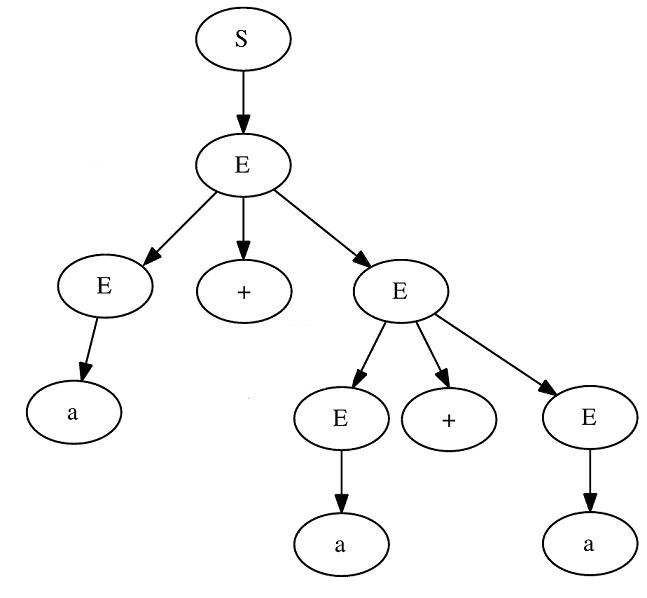
\includegraphics[width=5cm,height=6cm]{Pictures/div_tree1.jpeg}
	\label{fig:div_tree1}
\end{figure}

и

\begin{figure}[h]
	\centering
		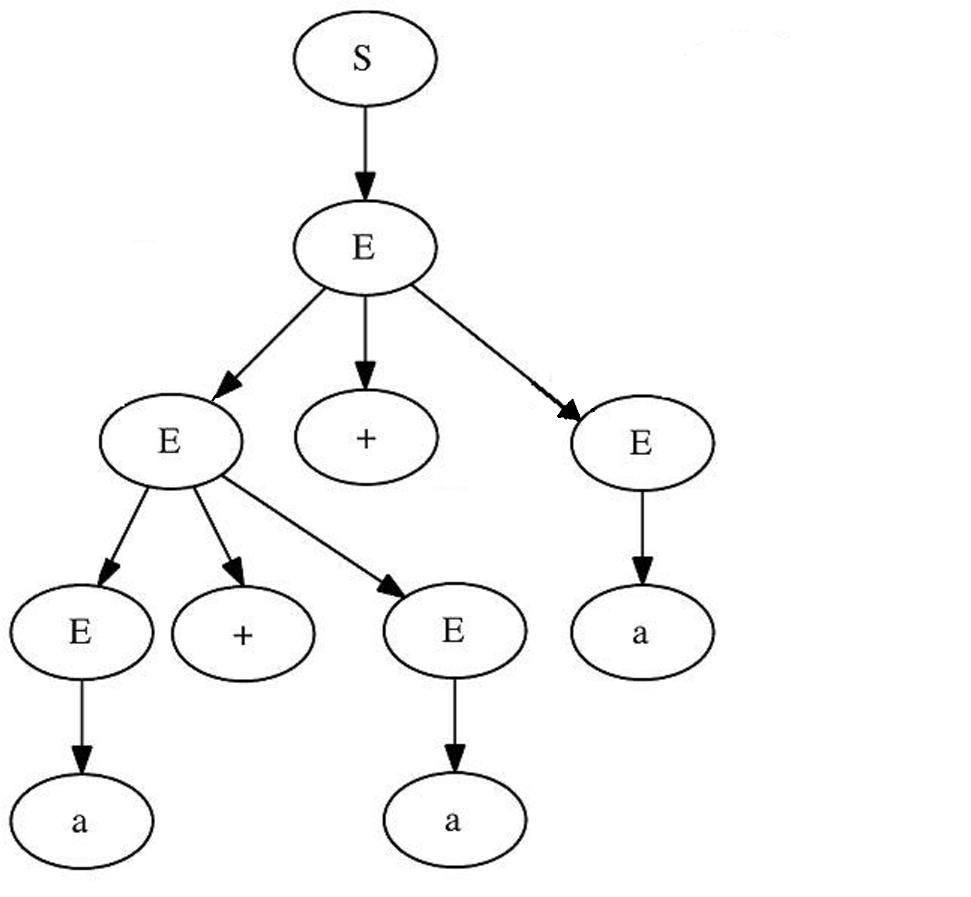
\includegraphics[width=5cm,height=6cm]{Pictures/div_tree2.jpeg}
	\label{fig:div_tree1}
\end{figure}
\clearpage
Соответственно, чтобы получить несколько деревьев вывода, необходимо расширить описанные выше функции так, чтобы они могли оперировать списками. 
 
 
